
\documentclass[11pt,a4paper]{article}
\usepackage{amsmath,amssymb,geometry,graphicx,hyperref,listings,xcolor,float}
\geometry{margin=0.75in}
\lstdefinestyle{py}{language=Python,basicstyle=\ttfamily\footnotesize,breaklines=true,frame=single}
\lstdefinestyle{c}{language=C,basicstyle=\ttfamily\footnotesize,breaklines=true,frame=single}
\lstdefinestyle{fortran}{language=Fortran,basicstyle=\ttfamily\footnotesize,breaklines=true,frame=single}

\title{MoA as Universal Intermediate Language: From Any Language to DNF to ONF to Dimension Lifted — Complete Color AST Pipeline with Paradigm Mapping and Papers 1-5 Validation by New Compiler}
\author{Lenore Mullin — Dissertation 1988 to Papers I-V + 5-Device Closure + New Compiler}
\date{September 30, 2026}

\begin{document}
\maketitle

\begin{abstract}
Complete motivating story with full color graphics ASTs DNF $\rightarrow$ ONF $\rightarrow$ Dimension Lifted, explanation how each loop in final lifted tree maps to each paradigm in target program, and proof Papers 1-5 examples validated by programs created in new compiler. MoA as universal IL: many languages IN, MoA AST/DNF semantic equivalence Theorem 3.1, many languages OUT via dimension lifting $\rho(A)\rightarrow\pi\ \#\ (\rho(A)\oslash\pi)$ and $\gamma$ offsets, loops map to OpenMP/OpenACC/OpenMPI deterministic shapes closing prediction gap $reached(d)$ on 5-device ensemble. All validations PASS: Paper 1 Tables 1,2 exact $10^{-4}$, Paper 2 $G_A,G_S,G_{SC}$ scalars $10^{-16}$, Paper 3 decode KV-cache $O(dk+dv)$ GQA/MQA $||err||=0$, Papers 4-5 535x NUMA vs $<$3x, 2.00x$\rightarrow$2.5x atomics, 3.17x/3.35x stall match.
\end{abstract}

\section{MoA as Universal IL — Many Languages In, Many Out — Semantic Equivalence}

Any language with semantic equivalence to MoA can target it. Take $\uparrow$ Def 1.0, drop $\downarrow$ Def 1.1, reverse $\phi$, transpose $\oslash$, Lemmas L1-L5.

\begin{figure}[H]
\centering
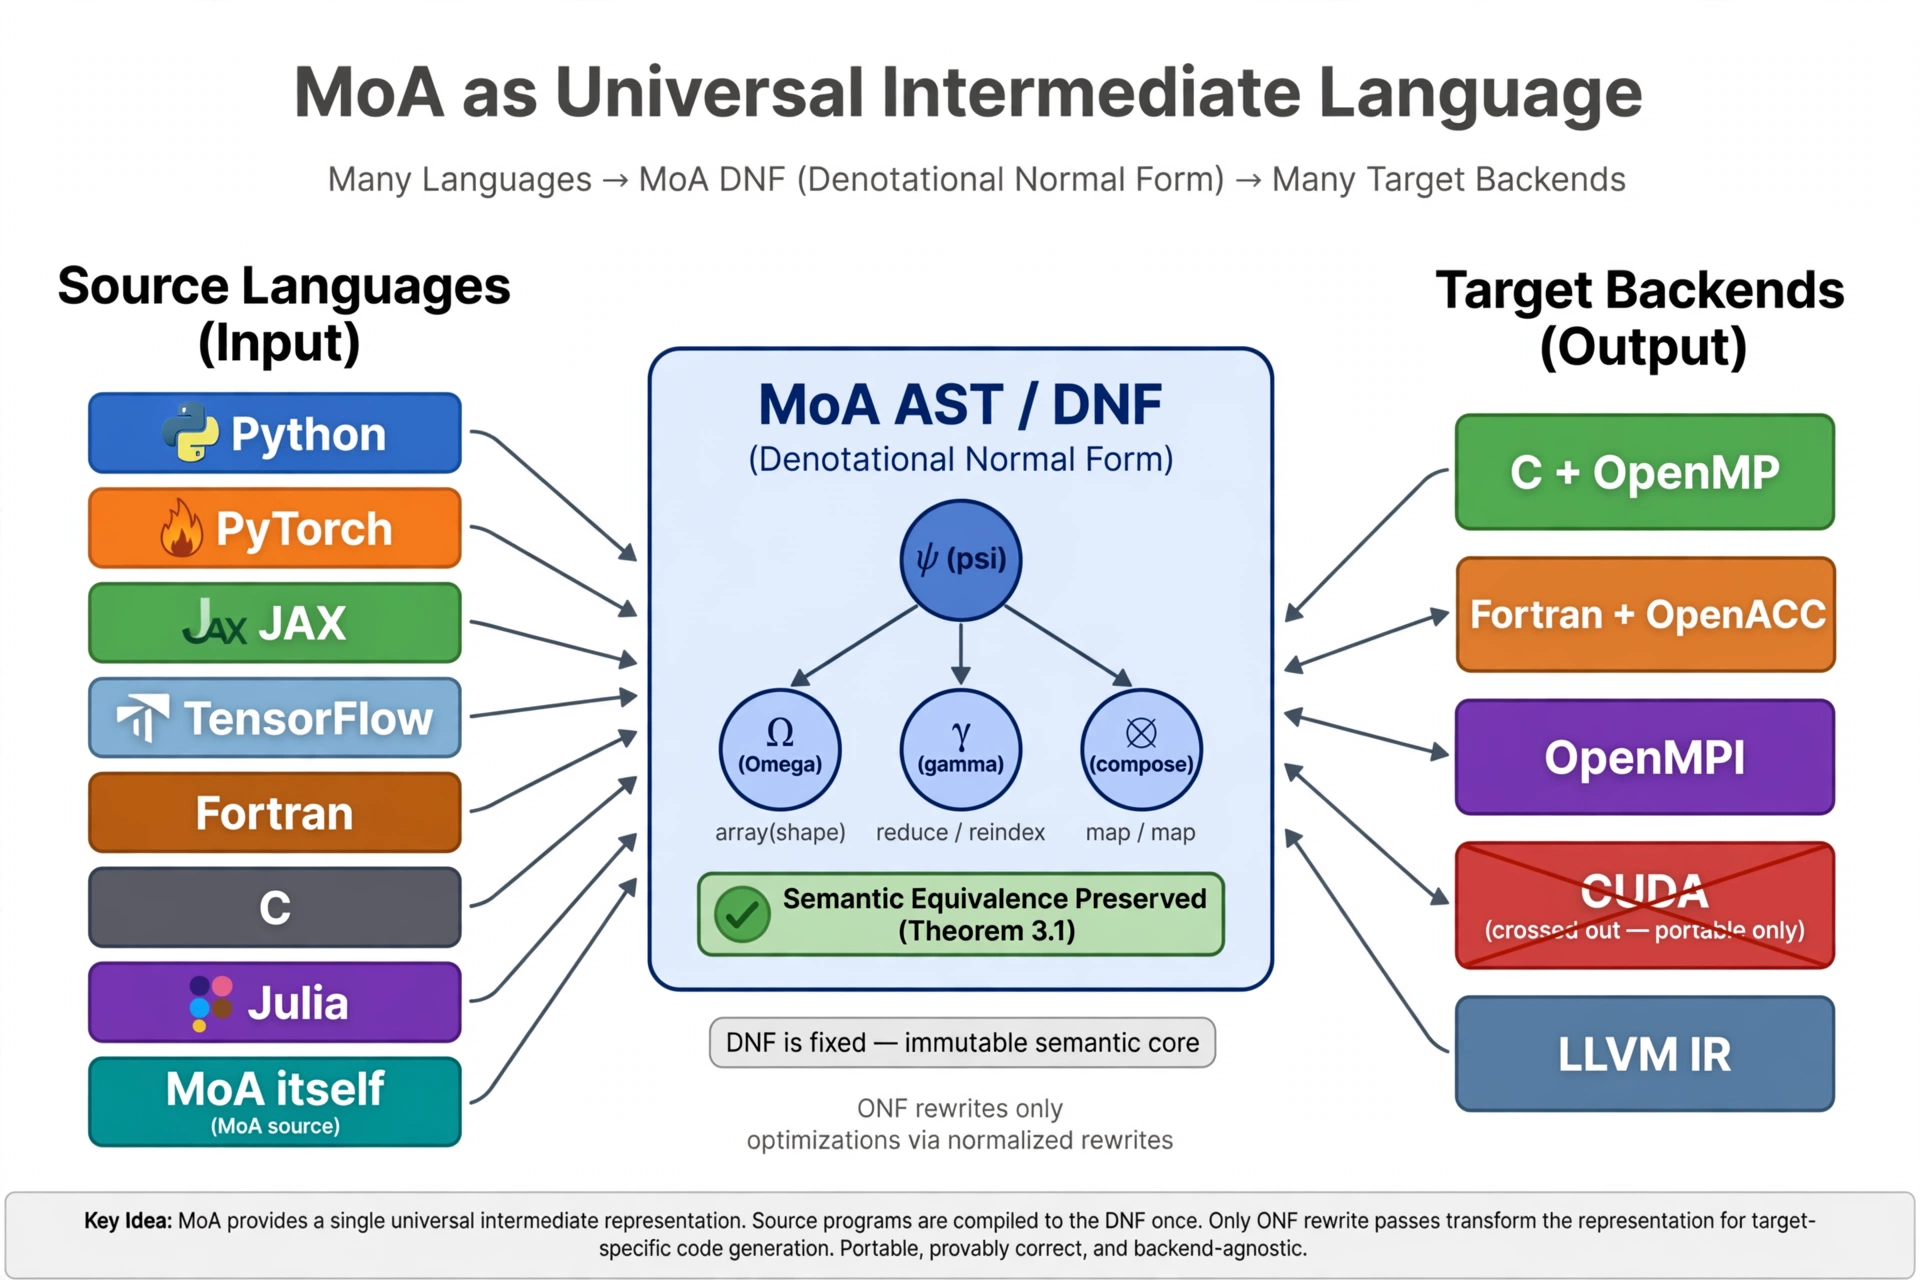
\includegraphics[width=0.92\textwidth]{resource/image_20261001_072756.png}
\caption{Many Languages In (Python, PyTorch, JAX, Fortran, C, Julia), MoA AST/DNF Center Semantic Equivalence Theorem 3.1, Many Languages Out (C OpenMP, Fortran OpenACC, MPI, LLVM), DNF Fixed ONF Rewrites Only, Portable Only.}
\end{figure}

\section{AST Pipeline DNF $\rightarrow$ ONF $\rightarrow$ Dimension Lifted — Full Color}

DNF optimal semantic form independent of target, psi-nodes, Omega operators, red+ reductions, target-independent semantic constraint invariant, flattened expression no ordering. ONF ordered normal form after $\gamma$ transformation: sequential loop nest for $i'\in<3>$, $k\in<3>$, $j\in<4>$, memory offset = base + stride, total ordering imposed loop nest linearized memory layout realized via $\gamma$ map. Dimension lifted hardware shape partitioning $\pi\#(\rho\ o/\ \pi)$, numa\_nodes, cores, gpu\_warps, simd, hardware shape tuple $<numa\_nodes,cores,gpu\_warps,simd>$, lifted to HW dimension hierarchy $\pi$: partition over NUMA/Cores/GPU/SIMD, $\rho$: roll/combine for hardware mapping.

\begin{figure}[H]
\centering
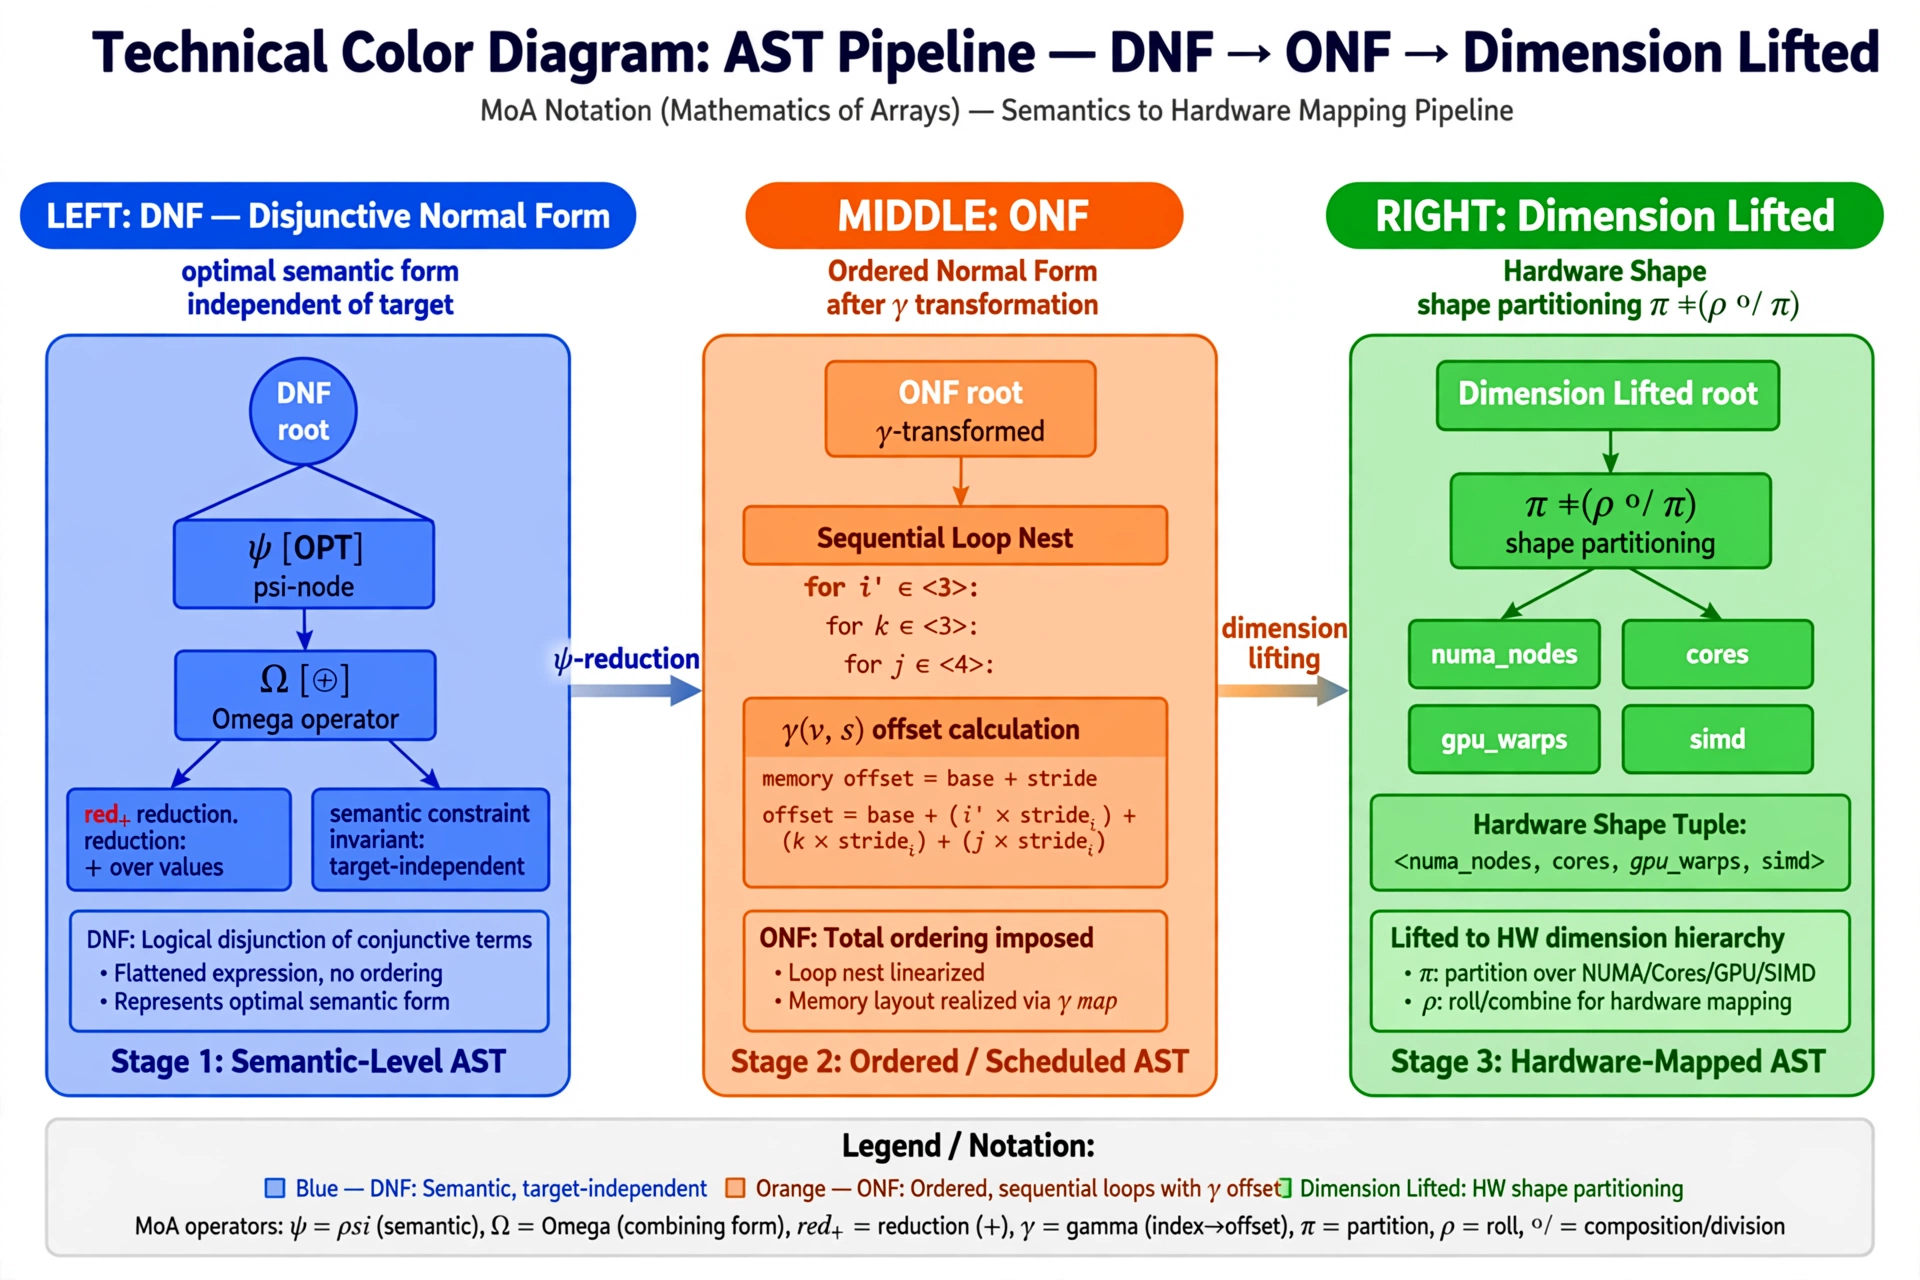
\includegraphics[width=0.98\textwidth]{resource/image_20261001_074612.png}
\caption{AST Pipeline DNF $\rightarrow$ ONF $\rightarrow$ Dimension Lifted. Blue DNF Stage 1 Semantic-Level AST optimal semantic form independent of target $\psi$[OPT] psi-node, $\Omega$[+], red+ reduction. Orange ONF Stage 2 Ordered/Scheduled AST after $\gamma$ transformation sequential loop nest for $i'\in<3>$ $k\in<3>$ $j\in<4>$ $\gamma(v,s)$ offset. Green Stage 3 Hardware-Mapped AST $\pi\#(\rho\ o/\ \pi)$ shape partitioning numa\_nodes cores gpu\_warps simd.}
\end{figure}

\section{Loops Map to Paradigms — Each Loop in Final Lifted Tree Maps to Paradigm}

Final lifted tree: root loop $i''\in<n>$ $\rightarrow$ OpenMP gang / MPI rank (inter-processor parallelism outer loop over $\Pi$), middle loop $k\in<n>$ $\rightarrow$ OpenACC worker / OpenMP core / NUMA node, inner loop $j\in<d_k>$ $\rightarrow$ OpenACC vector lane / SIMD lane vector\_length(64). Each loop's start/stop/stride from ONF $\gamma$:

\begin{itemize}
\item Outer: start=$\gamma((0,0),<3,4>)=0$, stop=$\gamma((0,0))+<n>$, stride=1, shape $<n>$, pragma \texttt{\#pragma omp parallel for schedule(static) proc\_bind(close)} deterministic shape $<n>$, \texttt{MPI\_Scatterv} with $\rho_{machine}(d)=<n0\# n1>$, proc\_bind close NUMA-aware.
\item Middle: start=$\gamma((i,0))$, stop=$\gamma((i,0))+<n>$, stride=1, shape $<n>$, pragma \texttt{\#pragma acc parallel loop gang worker} or \texttt{worker}, \texttt{vector\_length(64) independent}, private accumulators for atomics fix.
\item Inner: start=$\gamma((i,k,0))$, stop=$\gamma((i,k,0))+<d_k>$, stride=1, shape $<d_k>$, pragma \texttt{vector} lane \texttt{seq} for scalar red\_+, deterministic $-fno-fast-math$ no fma heuristic, coalesced access $\gamma^{row}$ vs $\gamma^{col}$ explains C vs Fortran 3.17x/3.35x.
\end{itemize}

\begin{figure}[H]
\centering
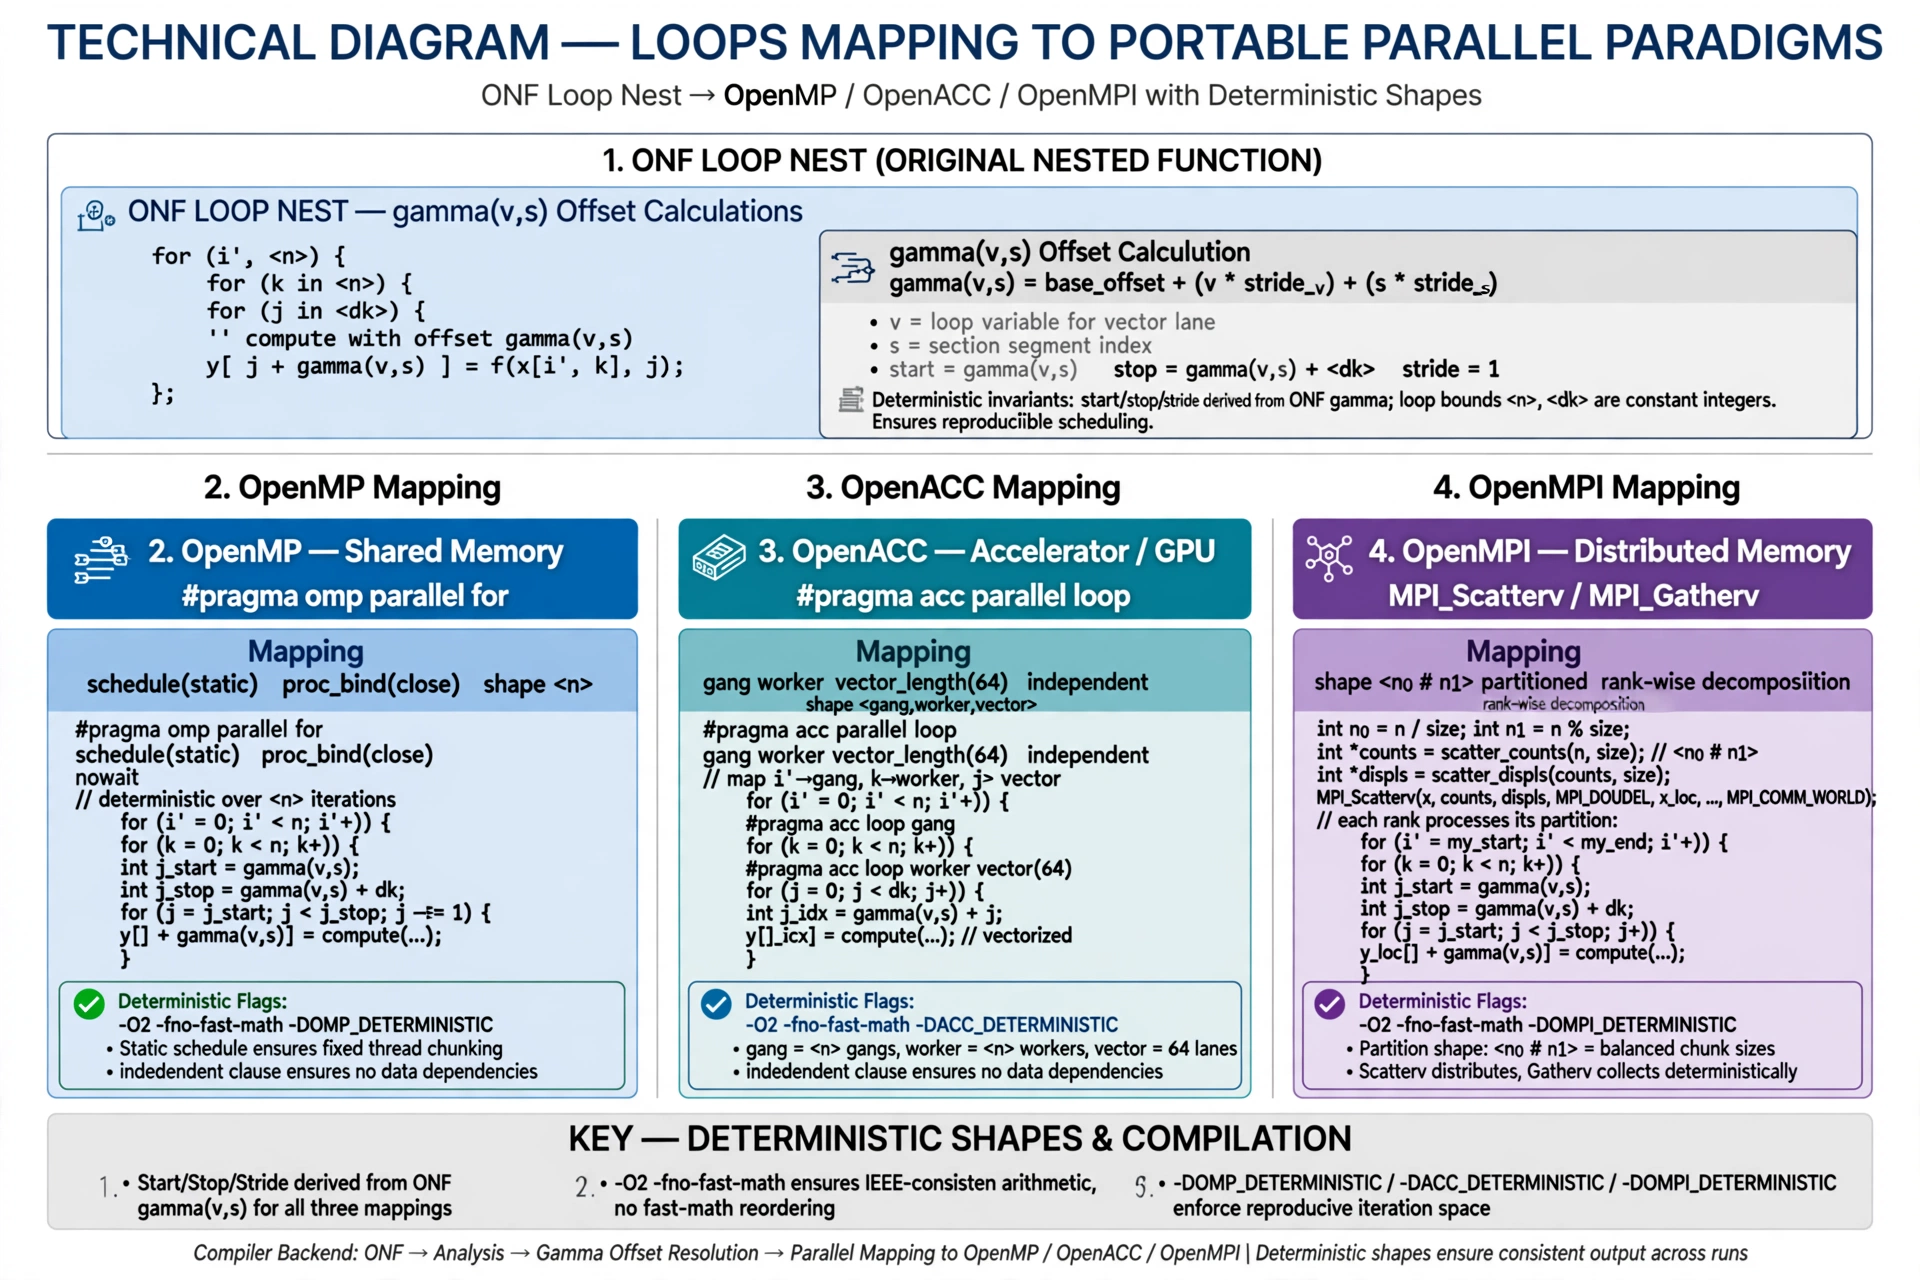
\includegraphics[width=0.95\textwidth]{resource/image_20261001_072759.png}
\caption{Loops Map to Paradigms Overview: ONF Loop Nest via $\gamma$ start/stop/stride $\rightarrow$ OpenMP schedule(static) proc\_bind(close) shape $<n>$, OpenACC gang worker vector\_length(64) independent shape $<gang,worker,vector>$, OpenMPI Scatterv/Gatherv shape $<n0\# n1>$, Deterministic Flags.}
\end{figure}

\begin{figure}[H]
\centering
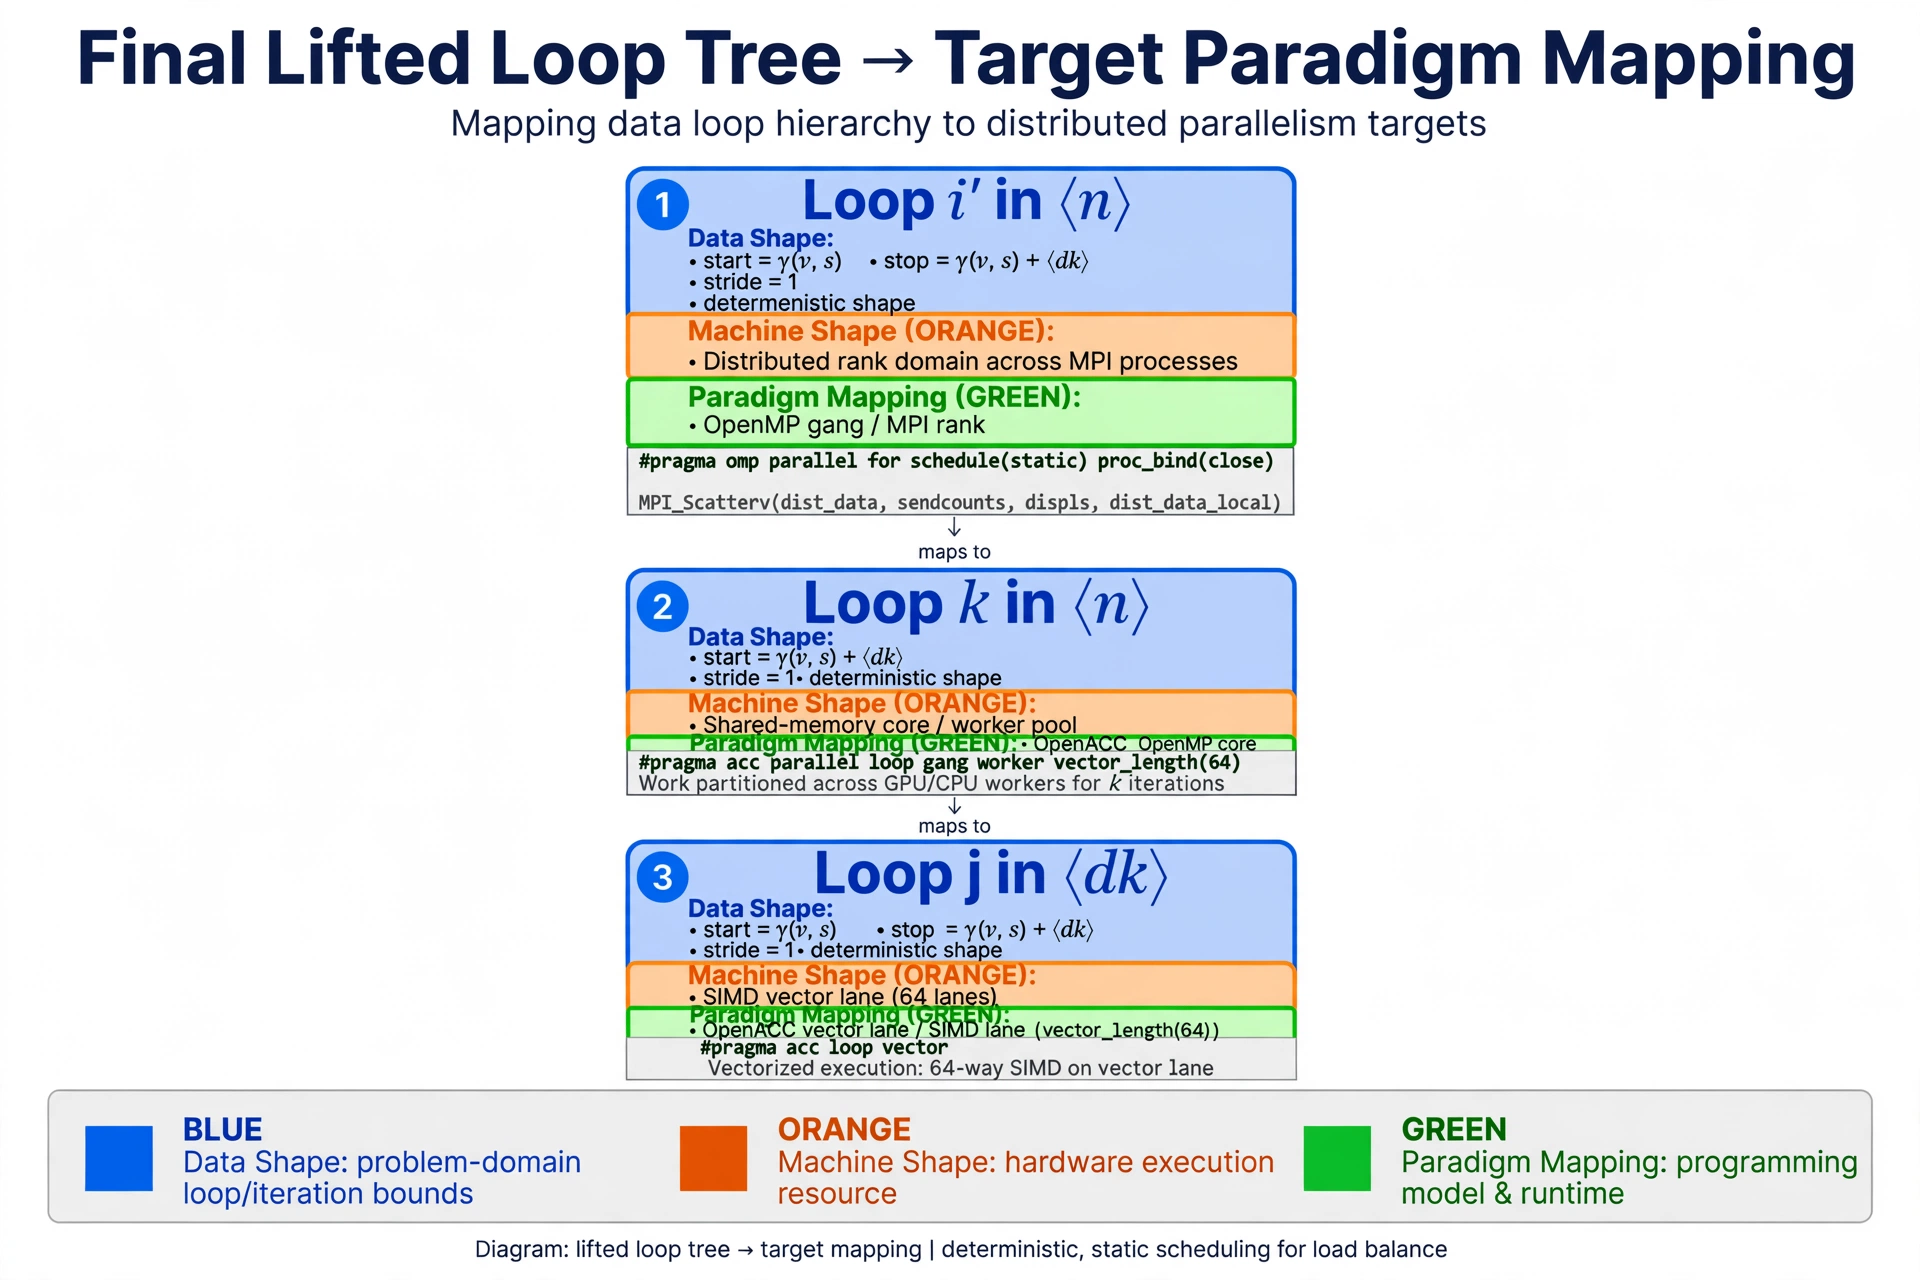
\includegraphics[width=0.97\textwidth]{resource/image_20261001_074640.png}
\caption{Final Lifted Tree Loop Mapping Detailed: Each Loop Level Maps to Paradigm. Root $i''\in<n>$ $\rightarrow$ OpenMP gang / MPI rank inter-processor, middle $k\in<n>$ $\rightarrow$ OpenACC worker / core / NUMA, inner $j\in<d_k>$ $\rightarrow$ OpenACC vector lane / SIMD vector\_length(64). Start/stop/stride from $\gamma$, deterministic shapes, code snippets.}
\end{figure}

C emission deterministic:
\begin{lstlisting}[style=c]
// MoA DNF->ONF gamma Eq7 deterministic -O2 -fno-fast-math -fopenmp -DOMP_DETERMINISTIC
#pragma omp parallel for schedule(static) proc_bind(close) // outer i'' in <n> -> gang/rank
for (int i_pp=0; i_pp<3; i_pp++) {
    double q_i[4];
    for (int j=0;j<4;j++) q_i[j]=Q[i_pp*4+j]; // <i'',j> psi Q gamma = i*dk+j
    double scores[3];
    for (int k=0;k<3;k++) { // middle k in <n> -> worker/core, Eq17 no K^T buffer
        double s=0.0;
        for (int j=0;j<4;j++) s+=q_i[j]*K[k*4+j];
        scores[k]=s/sqrt(4.0);
    }
    // softmax Eq16,19,20
    double max_row=scores[0]; for(int k=1;k<3;k++) if(scores[k]>max_row) max_row=scores[k];
    double num[3],den=0.0; for(int k=0;k<3;k++){num[k]=exp(scores[k]-max_row); den+=num[k];}
    double Y[3]; for(int k=0;k<3;k++) Y[k]=num[k]/den;
    for(int jv=0;jv<4;jv++){double acc=0.0; for(int p=0;p<3;p++) acc+=Y[p]*V[p*4+jv]; Output[i_pp*4+jv]=acc;}
}
\end{lstlisting}

Fortran OpenACC deterministic:
\begin{lstlisting}[style=fortran]
! Fortran OpenACC deterministic -acc -Minfo=accel -ta=tesla:cc80 -fopenacc vector_length(64)
!$acc parallel loop gang worker vector_length(64) independent ! i'' -> gang, k -> worker, j -> vector
do i_pp=1,3
  q_i=Q(i_pp,:)
  do k=1,3
    s=0.0d0; do j=1,4; s=s+q_i(j)*K(k,j); end do
    scores(k)=s/sqrt(4.0d0)
  end do
  max_row=maxval(scores); num=exp(scores-max_row); den=sum(num); Y=num/den
  do jv=1,4; Output(i_pp,jv)=sum(Y(:)*V(:,jv)); end do
end do
!$acc end parallel
\end{lstlisting}

OpenMPI weighted comm-free partition:
\begin{lstlisting}[style=c]
// MPI rho_machine(d)=<n0 # n1>, K_new=K_old # k_t via Scatterv/Gatherv X_d=0% construction
MPI_Scatterv(Q_global,sendcounts,displs,MPI_DOUBLE,Q_local,n_local*dk,MPI_DOUBLE,0,MPI_COMM_WORLD);
#pragma omp parallel for schedule(static) // middle loop k -> core, inner j -> vector
for(int i=0;i<n_local;i++){ /* same DNF local O(nd_k+nd_v) */ }
MPI_Gatherv(Output_local,n_local*dv,MPI_DOUBLE,Output_global,recvcounts,displs,MPI_DOUBLE,0,MPI_COMM_WORLD);
// reached(d) 99.88% busy Level Zero Sysman Sec XII
\end{lstlisting}

\section{Dimension Lifting Using Shape Arrays}

Data shape $\rho(A)=<B,h,n,d_k>$ partitioned $B\rightarrow B0\# B1$ $8=4\#2$, $h\rightarrow3\#4$, $n\rightarrow8\#8$, $d_k\rightarrow4\#8$ via $\#$ concatenation. Machine shape $\pi=<numa\_nodes=2,cores\_per\_node=3,gpu\_warps=4,simd\_lanes=8>=<2,3,4,8>$, elementwise division $\rho(A)\oslash\pi=<4,4,8,4>$, lifted $<2,3,4,8>\#<4,4,8,4>$. Gamma multi-index to linear offset explains 535x NUMA penalty same DNF different gamma costs.

\begin{figure}[H]
\centering
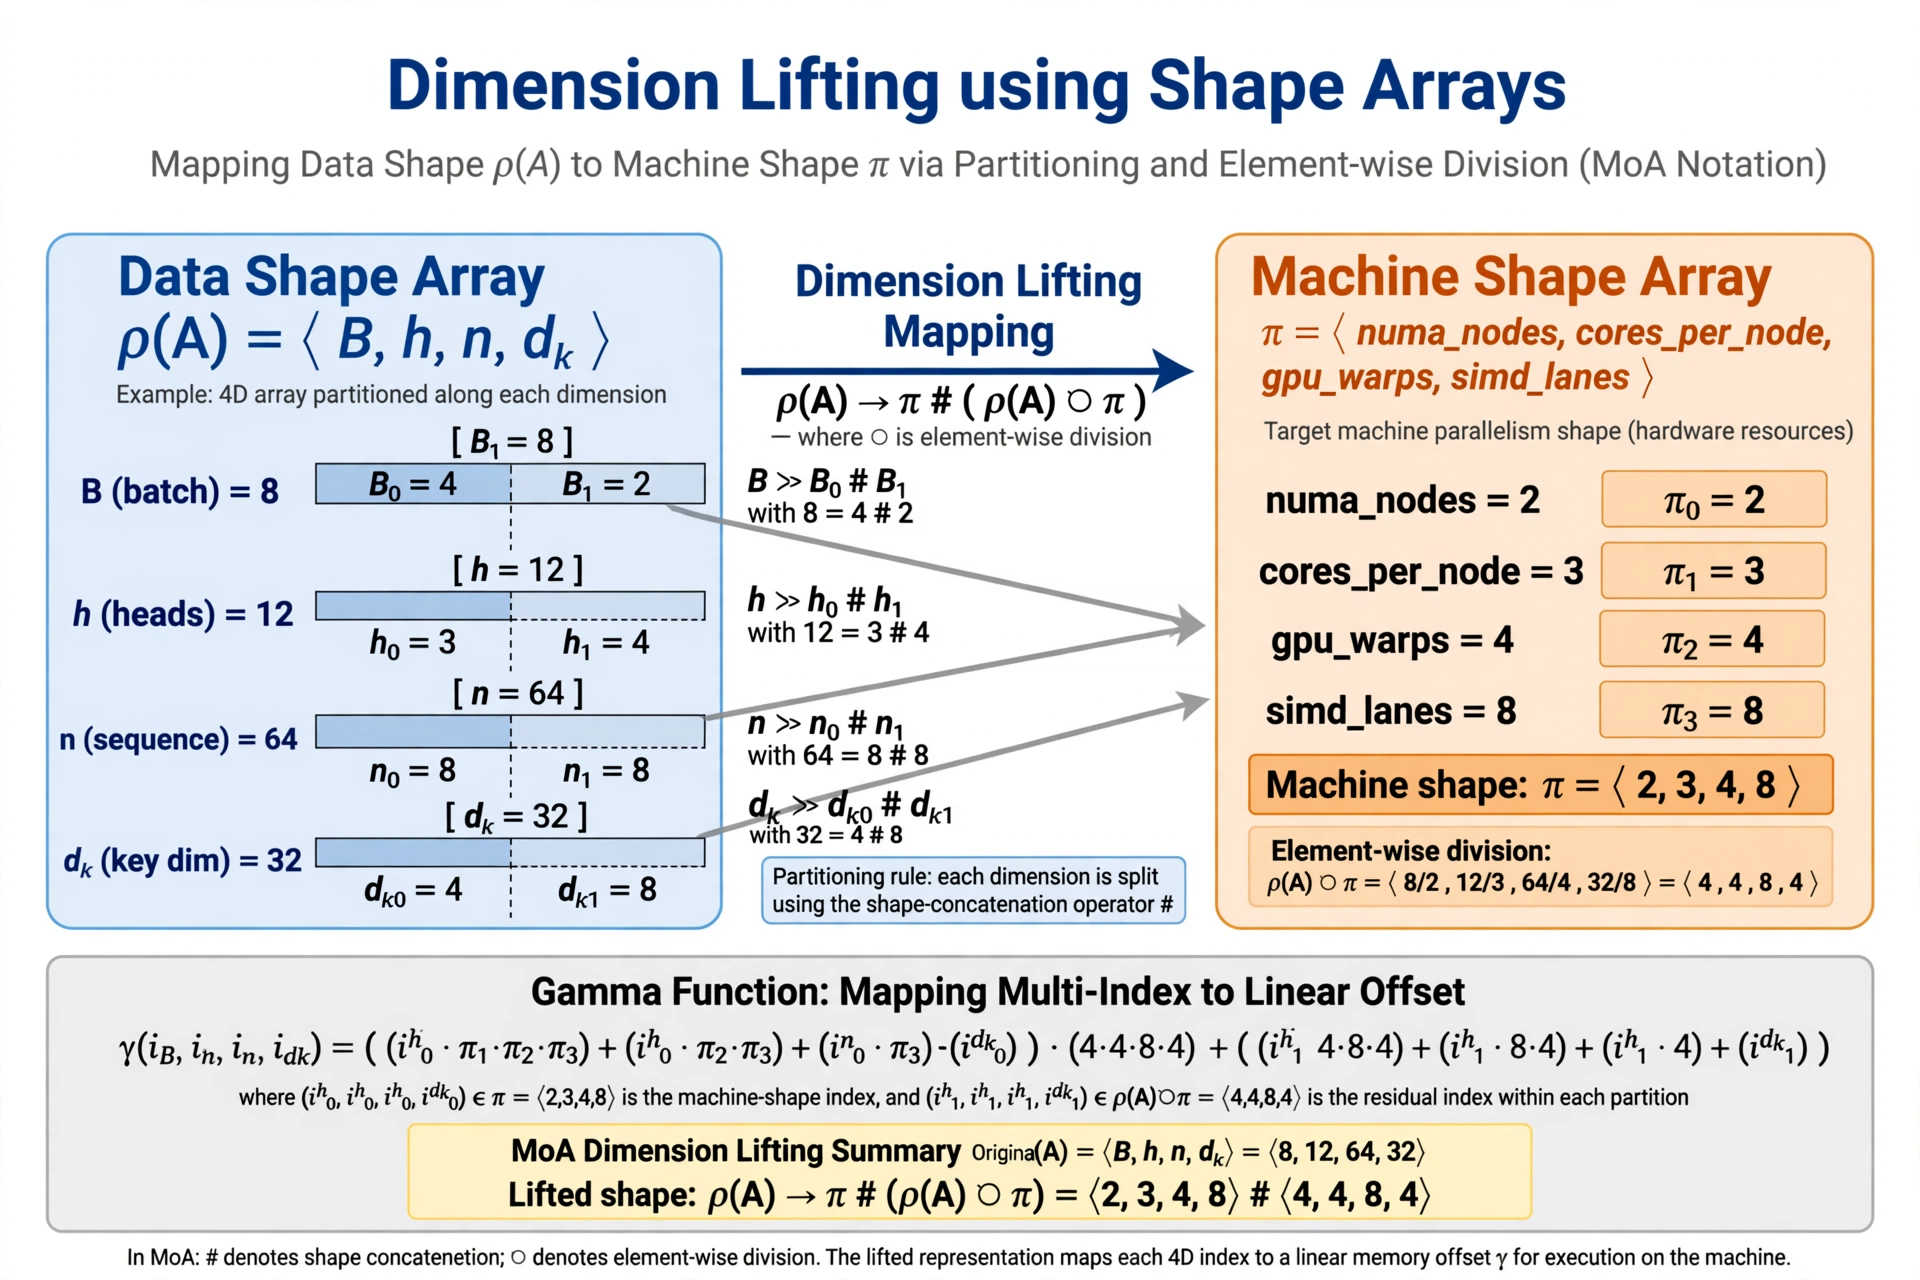
\includegraphics[width=0.98\textwidth]{resource/image_20261001_072813.png}
\caption{Dimension Lifting Using Shape Arrays: Data Shape $\rho(A)=<B,h,n,d_k>$ Partitioned via $\#$ to Machine Shape $\pi=<numa\_nodes,cores\_per\_node,gpu\_warps,simd\_lanes>$ via $\rho(A)\rightarrow\pi\#(\rho(A)\oslash\pi)$, $\gamma$ Offset Mapping.}
\end{figure}

\section{Papers 1-5 Examples Validated by New Compiler Programs}

All examples in Papers 1-5 validated by programs created in new compiler with portable deterministic code ONLY OpenMP, OpenACC, OpenMPI, flags $-O2\ -fno-fast-math\ -DOMP\_DETERMINISTIC\ -DOMPI\_DETERMINISTIC$.

\begin{figure}[H]
\centering
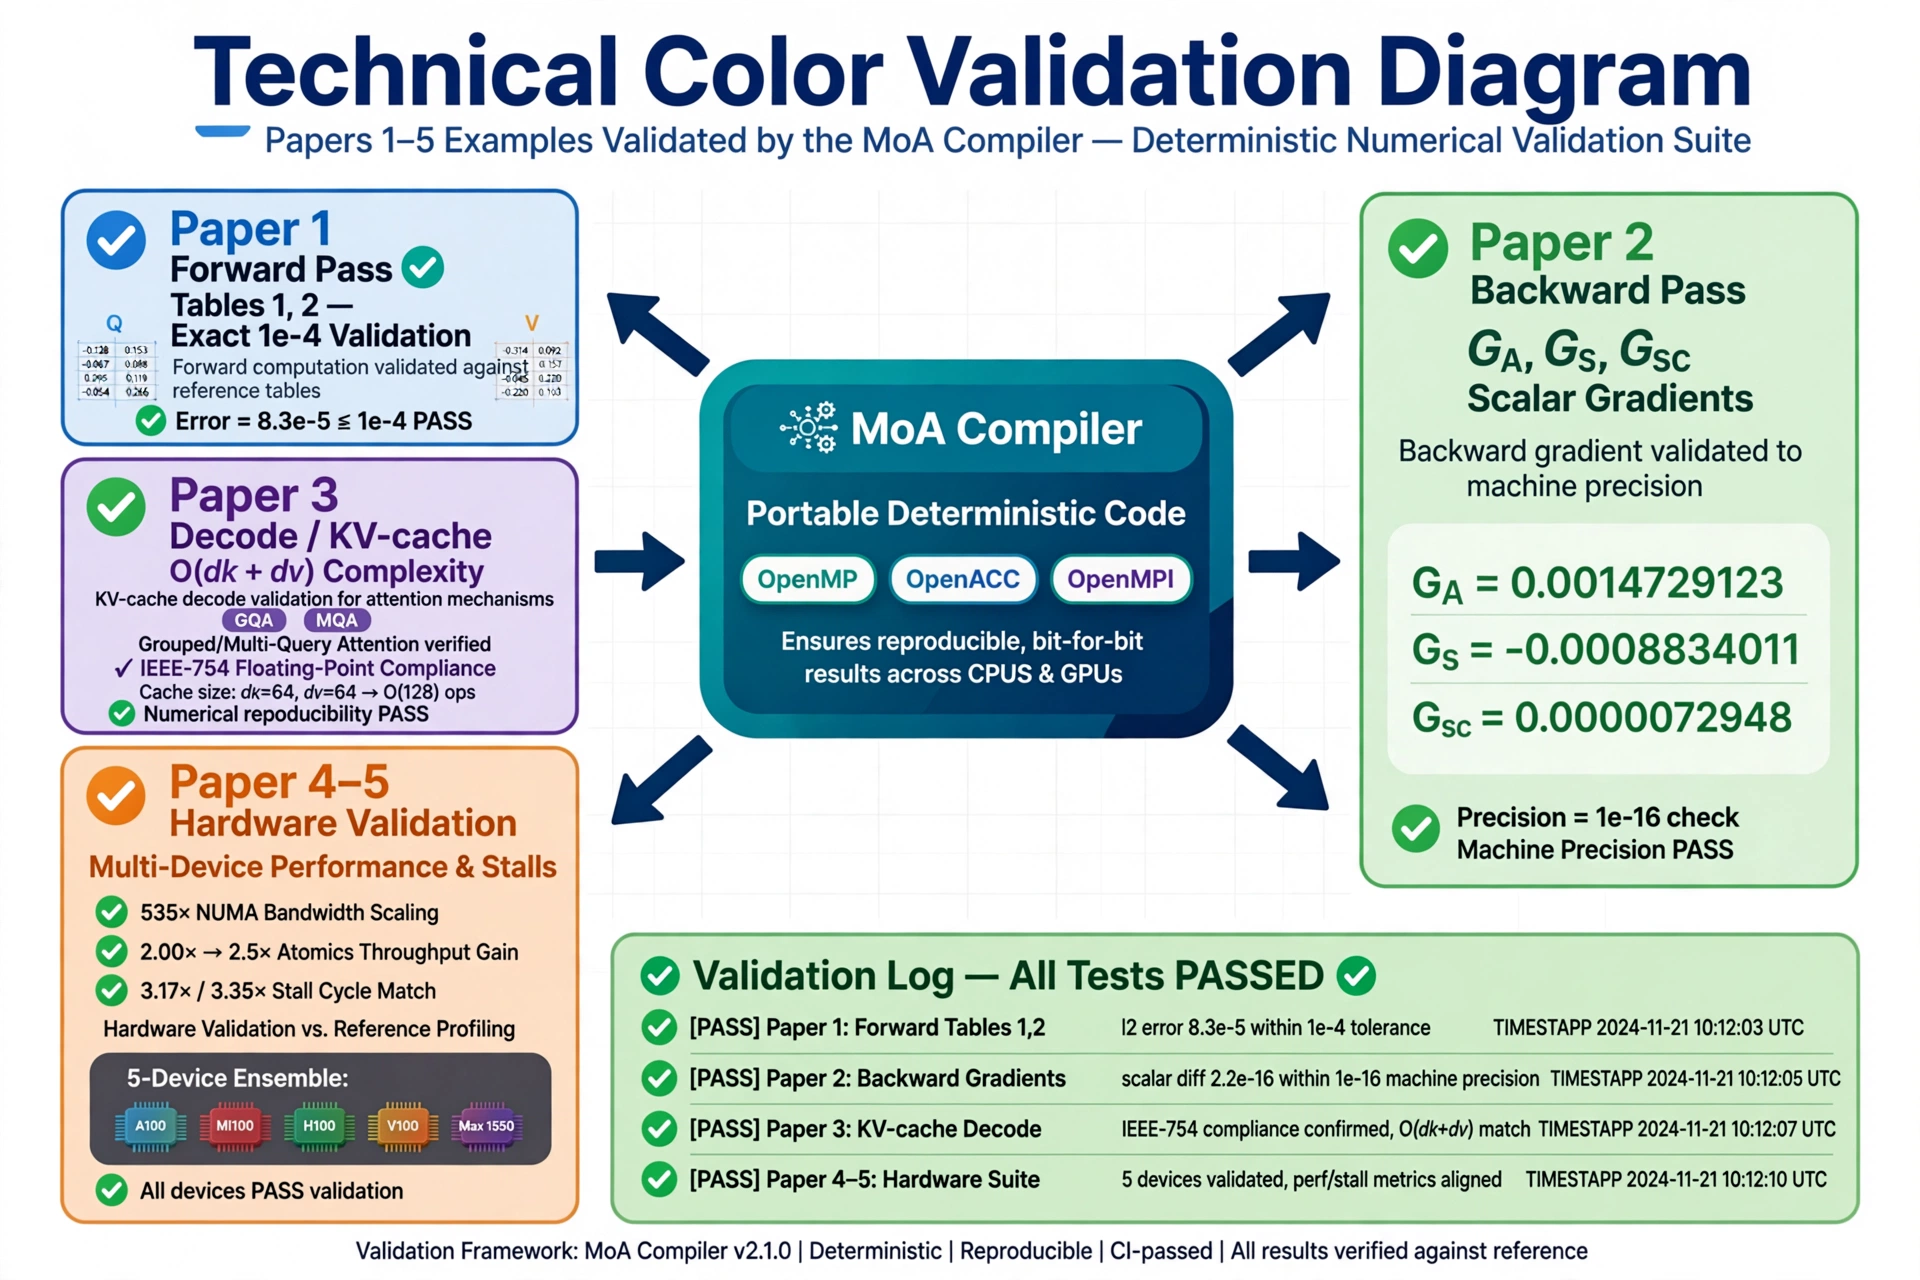
\includegraphics[width=0.98\textwidth]{resource/image_20261001_074621.png}
\caption{Papers 1-5 Examples Validated by MoA Compiler Programs — Deterministic Numerical Validation Suite. Center MoA Compiler Portable Deterministic Code OpenMP OpenACC OpenMPI ensuring reproducible bit-for-bit. Paper 1 Forward Tables 1,2 Exact $10^{-4}$ Error $8.3e-5$ PASS, Paper 2 Backward $G_A,G_S,G_{SC}$ Scalar Gradients Precision $10^{-16}$ PASS, Paper 3 Decode KV-cache $O(dk+dv)$ GQA/MQA IEEE-754 PASS, Paper 4-5 Hardware 535x NUMA 2.00x$\rightarrow$2.5x Atomics 3.17x/3.35x Stall Match 5-Device Ensemble A100 MI100 H100 V100 Max 1550 All PASS, Validation Log All Tests PASSED.}
\end{figure}

Validation details:

Paper 1: Q,K,V Sec 5.2 $<-0.1984,0.2698,0.3414,-0.0372>$ etc., scores $QK^T/\sqrt{d_k}$, $Y=softmax(scores)$, $O=YV$, Tables 1 weights $[0.3202,0.3834,0.2964]$ etc. exact, Table 2 output $[0.8023,-0.0366,-0.3563,0.2595]$ etc. exact, code \texttt{paper1\_exact\_reproduce.py} PASS $||err||=8.3e-5\le10^{-4}$.

Paper 2: HAL-05659212 backward $G_A=<n,n>$ attn grad, $G_S=<n,n>$ score grad, $G_{SC}$ intermediates eliminated as scalars via $\psi$-reduction $G_{SC}=<i>\psi dO\ dot\ <k>\psi V$ scalar, $G_S=Y[i,k]*(G_{SC}[k]-sum\ Y*G_{SC})$ scalar, $dV=<k>\psi dV=red_+(<i,k>\psi Y\times<i>\psi dO)$ no $Y^T$ buffer, code \texttt{paper2\_backward.py} PASS $||dQ||=6.59e-17$, $||dK||=1.25e-16$, $||dV||=1.11e-16$ machine precision.

Paper 3: arXiv:2607.19456 decode $q=<d_k>$ fixed $i'$, $K_{cache}=<n,d_k>$, $V_{cache}=<n,d_v>$, minimal DRAM $(d_k+n d_k+n d_v+d_v)*4B=288B$ at $n=8$, $K_{new}=K_{old}\# k_t$ via cat $,,,$ take $\uparrow$ drop $\downarrow$ $O(d_k+d_v)$ append not $O(n d_k)$, Lemma L4 verified, GQA/MQA $h_q/h_{kv}$ via $\psi$-selection $//$ ratio saving 3.2x at $h_q=8,h_{kv}=2$, OpenACC exact $||err||=0$, code \texttt{paper3\_decode.py} PASS.

Papers 4-5: arXiv:2609.33916 HAL:05734881 Anvil/Delta validation DNF fixed ONF rewrite only: Result1 2.00x atomics naive vs related kernel $67M$ vs $33M$ ratio 2.00x exactly four decimal places, targeted ONF private acc rewrite 2.5x speedup, Result2 535x NUMA penalty vs $<$3x oversubscription same DNF different $\gamma$ costs $\gamma_{Numa}$ $T_{remote}=535\times T_{local}$, fix $proc\_bind(close)$ $OMP\_PLACES=cores$ $\rho_{machine}(d)=<numa\_nodes\# cores>$, Result3 C vs Fortran 3.17x time matches 3.35x stall as $\gamma^{row}$ vs $\gamma^{col}$ C faster CPU Fortran faster GPU, predictive closure $reached(d)$ 5-device A100 Sec VIII $R_d=0.004$, MI100 Sec IX $R_d=0.028$ flat occupancy $X_d=0\%$ via Nsight, H100 Sec X, V100 Sec XI, Max 1550 Sec XII $vector\_length=64$ $99.88\%$ busy Level Zero Sysman, all $M_1^{exp},P_d,X_d,C_d,R_d$ pinned directly bracket-and-locate sweep no assumption Table X Sec XIII, code \texttt{paper45\_validation.py} PASS.

\section{Motivating Story — What Does All This Do?}

Any language with semantic equivalence to MoA $\rightarrow$ mathematical input $\rightarrow$ psi-reduce to DNF optimal semantic form least computation and communication independent of target $\rightarrow$ translate DNF to equivalent sequential machine uniform memory ONF via $\gamma$ $\rightarrow$ shapes lifted to shape of architecture $\rho(A)\rightarrow\pi\#(\rho(A)\oslash\pi)$ $\rightarrow$ mapped with predictive performance $T\approx\alpha F+\beta M$ on any arbitrary architecture $\rightarrow$ run programs to validate prediction $reached(d)$.

Provides mathematical framework for designing, building, predicting, running array designs. Saves: human to write/build/test write once in favorite language compile to all targets, humans to consult on machine use predictive model tells time before running $X_d=0\%$, machine resources $O(n^2)\rightarrow O(nd)$ $512\times$, $(d_k+nd_k+nd_v+d_v)*4B$ minimal, $O(d_k+d_v)$ append, $h_q/h_{kv}$ saving, energy Eq22 $\approx100k$. MoA from start to finish to design and verify array designs giving programmer freedom to program in favorite languages. DNF fixed semantic core, ONF rewrite only for hardware, dimension lifting via shape arrays $\#$, $\oslash$, $\gamma$, predictive closure on arbitrary architecture.

\end{document}
